\documentclass[dvipdfmx]{jsarticle}

\usepackage{ascmac}
\usepackage{url}
\usepackage[dvipdfmx]{hyperref}
\usepackage{pxjahyper}
\usepackage[dvipdfmx]{graphicx}
\usepackage{float}

\hypersetup{
  colorlinks=true,
  urlcolor=cyan
}

\begin{document}

\section{実験目的・課題}
次のデータを計算機上で表現し、
\begin{table}[h]
  \begin{tabular}{cccccc}
    Number & Name & Score0 & Score1 & Score2 & Score3 \\ \hline
    1 & Michael & 75 & 86 & 89 & 31 \\
    2 & Emma & 74 & 63 & 70 & 48 \\
    3 & Hannah & 73 & 45 & 82 & 31 \\
    4 & Emily & 40 & 30 & 49 & 48 \\
    5 & Daniel & 46 & 59 & 47 & 70
  \end{tabular}
\end{table}
\begin{itemize}
  \item ArrayListを使って名列番号順(Number)に表示
  \item Stackを使って名列番号の逆順に表示
  \item HashMapを使って名前(Name)の昇順に表示
  \item 名前と平均点を表示
  \item 平均点で昇順にソートして表示
  \item 名前がEで始まる学生だけを表示
\end{itemize}
を行う。

\section{実装方法}

  \subsection{方針}
  個人のNumber,Name,Score0...3をメンバにもつクラスを作成し、
  それをArrayListでまとめる。
  それを引数として与え、各課題の処理を行う関数を作成する。
  
  \subsection{成績クラス}
  メンバ変数としてNumber, Name, Scoresを持つクラスを作成する。
  それぞれの型はint, String, ArrayList$<$Integer$>$である。
  ScoresをArrayListにするのは今後成績が4つだけでなくそれより多く与えられる
  可能性も考えられるので可変長配列で受け取るのが今後そういった変更に対して
  対応しやすいためである。

  この3つの変数の初期値はコンストラクタで与え、
  今後変更されることはないとする。

  メンバ関数として、
  それぞれの変数の値を返す、
  Scoresの平均値を計算する、
  自身のデータを出力する、
  以上の3種類のものを用意する。

  \subsection{solve関数}
  \begin{description}
    \item[ArrayListを使って名列番号順(Number)に表示]\mbox{}\\
    ArrayList$<$成績クラス$>$を引数として受け取り、
    拡張for文でArrayListの要素それぞれに対して表示を行う。

    \begin{figure}[H]
      \centering
      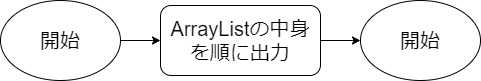
\includegraphics[width=0.9\hsize]{../pic/fc1.png}
      \caption{ArrayListを使って名列番号順に表示}
    \end{figure}

    \item[Stackを使って名列番号の逆順に表示]\mbox{}\\
    Stack$<$成績クラス$>$を宣言してそれにデータを前から順にプッシュする。
    それを順に取り出すとStackの構造上、プッシュしたときの逆順にデータを取り出すことが出来るので、
    その順に出力操作を行う。

    \begin{figure}[H]
      \centering
      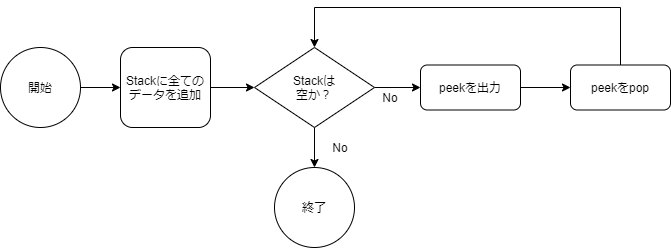
\includegraphics[width=0.8\hsize]{../pic/fc2.png}
      \caption{Stackを使って名列番号の逆順に表示}
    \end{figure}

    \item[HashMapを使って名前(Name)の昇順に表示]\mbox{}\\
    Stringをkey、成績クラスをvalueとしてもつHashMapを宣言し、
    データを拡張for文で順にHashMapに追加していく。
    このときに成績クラスのメンバ変数の値を取得するget\_Name()を使用する。
    同様にNameを取得してArrayList$<$String$>$に名前を追加する。
    この名前だけからなるArrayListを昇順にソートし、
    それに対して前から名前を取得していき、
    この名前でHashMapにアクセスすると、
    その人の成績クラスが帰ってくるので、
    それぞれでデータの出力を行う。

    \begin{figure}[H]
      \centering
      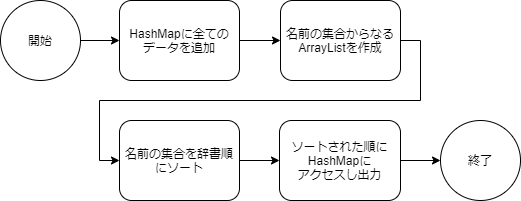
\includegraphics[width=13cm]{../pic/fc3.png}
      \caption{HashMapを使って名前(Name)の昇順に表示}
    \end{figure}

    \item[名前と平均点を表示]\mbox{}\\
    拡張for文でデータを舐め、
    それぞれで平均点を計算して、
    出力を行う。

    平均点は成績のデータ数を$N$として
    $\displaystyle \frac{1}{N} \sum_{i=0}^{N-1} Scores_i$
    で計算できる。

    \begin{figure}[H]
      \begin{center}
        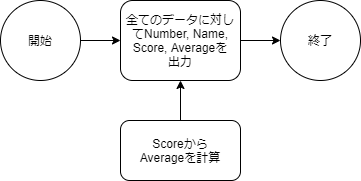
\includegraphics[width=10cm]{../pic/fc4.png}
        \caption{名前と平均点を表示}
      \end{center}
    \end{figure}

    \item[平均点で昇順にソートして表示]\mbox{}\\
    java.util.Collectionsをimportすることで
    Collections.sort()が使えるようになる。
    この関数は、データと比較クラスを引数として与えることで
    比較クラスに基づいてデータをソートをすることが出来る。
    
    今回は平均点の昇順にソートしたいので、
    成績クラス$S_1, S_2$を引数にとり、
    それぞれでget\_average()によって平均値を計算し、
    その値同士で比較をするcomparatorクラスを作成した。

    \begin{figure}[H]
      \centering
      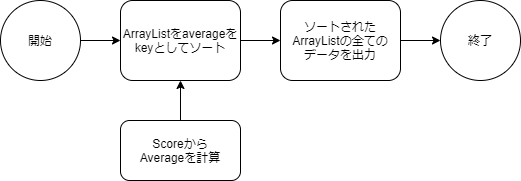
\includegraphics[width=15cm]{../pic/fc5.png}
      \caption{平均点で昇順にソートして表示}
    \end{figure}

    \item[名前がEで始まる学生だけを表示]\mbox{}\\
    拡張for文でデータを舐め、
    それぞれでget\_Name().charAt(0)で
    名前の初めの文字を取得し、
    それが'E'と等しければデータを出力する。

    \begin{figure}[H]
      \begin{center}
        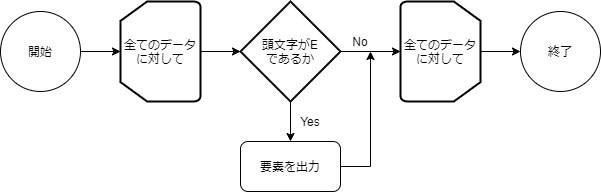
\includegraphics[width=15cm]{../pic/fc6.png}
        \caption{名前がEで始まる学生だけを表示}
      \end{center}
    \end{figure}
    
  \end{description}

\section{結果と考察}

\subsection{ArrayListを使って名列番号順(Number)に表示}
結果を以下に示す。
\begin{screen}
  1   Michael 75,86,89,31,\\
  2      Emma 74,63,70,48,\\
  3    Hannah 73,45,82,31,\\
  4     Emily 40,30,49,48,\\
  5    Daniel 46,59,47,70,
\end{screen}

出力の左端の名列番号をみると、
1,2,3,4,5の順になっていることから
この出力は正しいと考えらえる。
\subsection{Stackを使って名列番号の逆順に表示}
結果を以下に示す。
\begin{screen}
  5    Daniel 46,59,47,70,\\
  4     Emily 40,30,49,48,\\
  3    Hannah 73,45,82,31,\\
  2      Emma 74,63,70,48,\\
  1   Michael 75,86,89,31,
\end{screen}

出力の左端の名列番号をみると、
5,4,3,2,1の順、つまり先の逆順になっていることから
この出力は正しいと考えらえる。

\subsection{HashMapを使って名前(Name)の昇順に表示}
結果を以下に示す。
\begin{screen}
  5    Daniel 46,59,47,70,\\
  4     Emily 40,30,49,48,\\
  2      Emma 74,63,70,48,\\
  3    Hannah 73,45,82,31,\\
  1   Michael 75,86,89,31,
\end{screen}

学生を辞書順で並べると
Daniel $<$ Emily $<$ Emma $<$ Hannah $<$ Michael
であり、出力と比べると一致しているため、
この出力は正しいと言える。

\subsection{名前と平均点を表示}
結果を以下に示す。 
\begin{screen}
  1   Michael 75,86,89,31, 70\\
  2      Emma 74,63,70,48, 63\\
  3    Hannah 73,45,82,31, 57\\
  4     Emily 40,30,49,48, 41\\
  5    Daniel 46,59,47,70, 55
\end{screen}

実際にMichaelの平均点を計算すると、
$\displaystyle \frac{75+86+89+31}{4} = \frac{281}{4} = 70.25$
と結果と一番右端の数字が一致しているため、
この出力は正しいと考えられる。
しかし、Michaelの平均点は70.25だが、
表示されている点数は70点になっている。これは、
平均点をintで計算しているため、
割り算をするときに小数点以下が切り捨てされるためである。

今回の実装では点数の和を先に計算して、
最後にNで割っているため小数点以下の切り捨てが
一度しか起こらないため誤差は1未満になる。もし、
$\displaystyle \sum_{i=0}^{N-1} \frac{Scores_i}{N}$
のように計算すると、
誤差の量は
$\displaystyle \sum_{i=0}^{N-1} \frac{Scores_i \% N}{N}$
のように計算出来て、
最悪N-1点の誤差が生まれることになる。

\subsection{平均点で昇順にソートして表示}
結果を以下に示す。
\begin{screen}
  4     Emily 40,30,49,48, 41\\
  5    Daniel 46,59,47,70, 55\\
  3    Hannah 73,45,82,31, 57\\
  2      Emma 74,63,70,48, 63\\
  1   Michael 75,86,89,31, 70
\end{screen}

平均点を上から見ていくと小さい順に並んでいることがわかる。
つまりこの出力は正しいと考えられる。

この平均点のソートには学生の数をN、スコアの数をMとして、
O(MNlogN)かかっている。
ソートはO(NlogN)だが今回は比較のたびに
O(M)かけて点数の平均値を計算しているためである。
例えばコンストラクタでスコアを受け取った時に
平均値を計算しておくなどすれば平均値の取得がO(1)で
できるようになり、O(NlogN)で処理を完了できる。
ここからさらにオーダーを改善することもでき、
テストの平均値としてありうる値の範囲を[0,A]の整数値
とするとバケットソートでO(N+A)で計算できる。

\subsection{名前がEで始まる学生だけを表示}
結果を以下に示す。
\begin{screen}
  4     Emily 40,30,49,48,\\
  2      Emma 74,63,70,48, 
\end{screen}

Daniel,Hannah,Michaelは名前がEで始まる学生ではないので
表示されないのが正しい。
つまりこの出力も正しいと考えられる。

ここで、学籍番号が4,2の順番で表示されている。
最初に宣言したときは1,2,3,4,5の順番であり、main関数内では
データを変更していないのでこうなるのは不自然である。
これは、平均値でソートしたときにデータが変更されたのが原因である
と考えられる。それは、
javaには値渡ししか存在しないがプリミティブ型以外の型では
ほかの言語でいうところの参照渡しと似た挙動をするためである。

\begin{thebibliography}{10}
  \bibitem{1} ArrayList 要素のソートと Comparator 
  
  \url{https://java.keicode.com/lib/collections-sort.php}
  
  \bibitem{2} もう参照渡しとは言わせない 
  
  \url{https://qiita.com/mdstoy/items/2ef4ada6f88341466783}
\end{thebibliography}

\end{document}